\documentclass[a4paper,oneside, 12pt]{article}

\usepackage[margin=0.7in]{geometry}
\usepackage[cm-default]{fontspec}
\usepackage{xunicode}
\usepackage{xltxtra}
\usepackage{xgreek}
\usepackage{graphicx}
\graphicspath{{../UML/}{UML/}}

\setmainfont[Mapping=tex-text]{Linux Libertine O}

\title{Stakeholders Requirements Specification\\
\begin{flushleft}
	Εθελοντής
\end{flushleft}}
\date{\vspace{-5ex}}

\begin{document}
\maketitle
\section{Εισαγωγή}
\subsection{Ταυτότητα-επιχειρησιακοί στόχοι}

Το παρόν έργο αφορά την υλοποίηση μιας εφαρμογής παρατητηρίου, που θα επιτρέπει 
σε χρήστες εθελοντές να ενημερώνουν την κοινότητα για προσφορές υγρών καυσίμων 
μέσω ηλεκτρονικών αναρτήσεων. Στόχος του εθελοντή ως συμμέτοχου αποτελεί η 
συγκέντρωση πόντων στα πλαίσια της εφαρμογής και επιβραβεύσεων που παρέχονται 
από τους καταστηματάρχες ως συμμέτοχοι. Επιπλέον, επιχειρησιακός στόχος είναι 
και η ανιδιοτελής προσφορά στο κοινωνικό σύνολο. Ο εθελοντής επισκέπτεται τα 
πρατήρια υγρών καυσίμων που συμμετέχουν στην εφαρμογή και αναφορά τιμών και 
εκπτώσεων για προβολή από άλλους καταναλωτές.

\subsection{Περίγραμμα επιχειρησιακών λειτουργιών}

Ο εθελοντής έχει τη δυνατότητα να χρησιμοποιήσει την εφαρμογή για να κάνει 
εισαγωγή δεδομένων, επιλέγοντας ένα προϊόν και σε περίπτωση που ήδη υπάρχει 
να κάνει καταχώριση μιας νέας τιμής για το συγκεκριμένο προϊόν. Διαφορετικά, 
μπορεί να εισάγει το καινούριο προϊόν στη βάση δεδομένων, ώστε να γίνουν 
τυχόν περαιτέρω παρατηρήσεις πάνω στις διακυμάνσεις της τιμής στο μέλλον. 
Επιπλέον, ο χρήστης μπορεί να πάρει πληροφορίες από το σύστημα, εισάγοντας 
δικές του παραμέτρους και εκτελώντας αναζήτηση. Αυτά φαίνονται στο παρακάτω 
UML διάγραμμα.

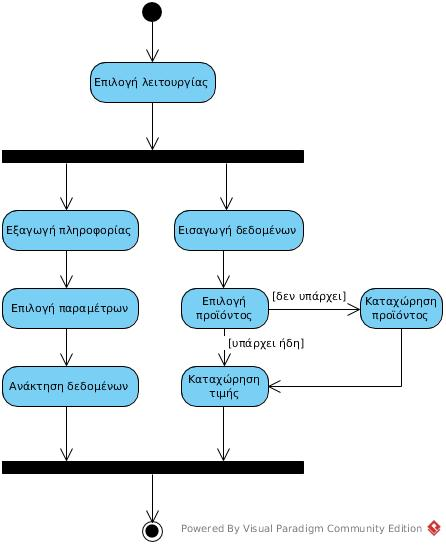
\includegraphics[scale=0.6]{UML-01}

\section{Αναφορές-πηγές πληροφοριών}

Ν/Α

\section{Διαχειριστικές απαιτήσεις επιχειρησιακού περιβάλλοντος}
\subsection{Επιχειρησιακό μοντέλο}
Το επιχειρησιακό μοντέλο βασίζεται στην επιθυμία του καταστηματάρχη να 
επιβραβεύσει την προβολή των προϊόντων του, και σε εκπτώσεις που διενεργούνται. 
Ειδικότερα, τα πρατήρια υγρών καυσίμων αποσκοπούν στην προσέλκυση επιπλέον πελατών 
και για αυτό είναι διατεθειμένα να επιβραβεύσουν τους εθελοντές. Συνεπώς, ο 
εθελοντής θα λάβει μειώσεις τιμών από τα καταστήματα που κατέγραψε την τιμή τους 
ως ενθάρρυνση για περαιτέρω συμμετοχή στο πληθοποριστικό οικοσύστημα. 

\subsection{Περιβάλλον διαχείρισης πληροφοριών}

N/A

\section{Λειτουργικές απαιτήσεις επιχειρησιακού περιβάλλοντος}
\subsection{Επιχειρησιακές διαδικασίες}
Ο εθελοντής συνδέεται στην εφαρμογή και μέσω διαισθητικής διεπαφής δηλώνει 
τη τιμή του εκάστοτε προϊόντος. Ταυτόχρονα δηλώνει σε ένα χάρτη τη τοποθεσία 
της προσφοράς, ώστε να μαθευτεί σε άλλου χρήστες της εφαρμογής. Επιπλέον, η 
αναφορά του μπορεί να βαθμολογηθεί από άλλους χρήστες για την ακρίβεια της, με στόχο την ανάδειξη των καλύτερων και πιο ακριβών αναφορών. Σε περίπτωση που οι αναφορές για ένα συγκεκριμένο πρατήριο από έναν χρήστη έχουν ιδιαίτερη αναγνώριση ο χρήστης λαμβάνει επιβραβεύσεις στη μορφή πόντων από το εκάστοτε κατάστημα.

\subsection{Περιορισμοί}

Ο χρήστης πρέπει κατ’αρχάς να βρίσκεται στη συγκεκριμένη τοποθεσία για να εκτελέσει καταγραφή της εκάστοτε τιμής ή να επιβεβαιώσει/διαψεύσει κάποια ήδη υπάρχουσα τιμή. Επιπλέον πρέπει να είναι διατεθειμένος να παρέχει τα σχετικά διαπιστευτήρια ώστε να πιστοποιηθεί ως ο συγκεκριμένος χρήστης και να αποφευχθεί η πλαστοπροσωπία και η κακόβουλη χρήση της εφαρμογής  

\subsection{Δείκτες ποιότητας}
Ο εθελοντής αξιολογεί την εφαρμογή με βάση δείκτες ποιότητας όπως η ευχρηστία, η αποδοτικότητα καθώς και άλλες μετρικές όπως η αποκρισιμότητα. Επιπλέον, επιθυμεί η εφαρμογή να του επιτρέπει γρήγορη και αποτελεσματική δυνατότητα αναφοράς σημαντικών προσφορών σε τυχόν καταστήματα που συμμετέχουν στην εφαρμογή. Ποσοτικά ο χρήστης ελέγχει το κατά πόσο η χρήση της εφαρμογής είναι ευχάριστη και χωρίς εμπόδια, εκτελώντας ταυτόχρονα την επιθυμητή λειτουργία.

\section{Έκθεση απαιτήσεων χρηστών}
Στις λειτουργικές απαιτήσεις του εθελοντή συγκαταλέγονται η δυνατότητα του να εκτελέσει καταγραφή των τυχόν προσφορών. Επιπλέον, περιλαμβάνεται και η ύπαρξη ενός συστήματος αναγνώρισης της αξίας των αναφορών των εκάστοτε προσφορών. Οι εθελοντές πρέπει να μπορούν να δουν σε μια χωρική απεικόνιση την τοποθεσία τους, καθώς και τη τοποθεσία του προϊόντος που καταγράφουν. Αυτό σημαίνει ότι το σύστημα πρέπει υποχρεωτικά να τους παρέχει τη δυνατότητα να οπτικοποιήσουν την τοποθεσία της καταγραφής με χρήση χαρτών. Περαιτέρω, οι χρήστες/εθελοντές απαιτείται να έχουν τη δυνατότητα εξελιγμένης αναζήτησης, ώστε να μπορούν να βρουν τι είναι ήδη καταγεγραμμένο και αν υπάρχει δυνατότητα ενημέρωσης της τιμής κάποιου υπάρχοντος προϊόντος. Τέλος, είναι αναγκαίο να μπορούν να κάνουν καταγγελία (report) κάποιας υπάρχουσας εγγραφής, δηλαδή εγγραφής που δεν ανταποκρίνεται στην πραγματικότητα.

Στις μη λειτουργικές απαιτήσεις ανήκουν η ανάγκη για χρηστικότητα και αποδοτικότητα του συστήματος. Το σύστημα πρέπει να έχει αξιόπιστο uptime και να είναι διαθέσιμο τις περισσότερες φορές. Ακόμα, κρίνεται αναντικατάστατη η ύπαρξη ασφάλειας και προστασίας των δεδομένων του χρήστη από κακόβουλους παράγοντες.   

\section{Αρχές του προτεινόμενου συστήματος}

Η υπηρεσία είναι μια διαδικτυακή εφαρμογή που παρέχει τη δυνατότητα καταγραφών τιμών από εθελοντές χρήστες. Από την πλευρά του εθελοντή στο παρατηρητήριο  τοποθετούνται δεδομένα τα οποία επιβεβαιώνονται από άλλους χρήστες ή διαψεύδονται όταν οι τιμές αλλάξουν. Δίνει τη δυνατότητα στους εθελοντές να εισπράξουν πόντους ως επιβράβευση για τη συμβολή τους, τους οποίους μπορούν να εξαργυρώσουν ως εκπτώσεις στο εκάστοτε κατάστημα. 

Η εφαρμογή επιτρέπει στους εθελοντές-χρήστες τη δυνατότητα οπτικοποίησης της τοποθεσίας των υπαρχόντων δεδομένων με χρήση υπηρεσίας χαρτών. Τέλος υπάρχει η δυνατότητα προηγμένου συστήματος αναζήτησης.

\section{Περιορισμοί στο πλαίσιο του έργου}

Στο πλάισιο του έργου οι εθελοντές επιβάλλουντους εξής περιορισμους. Πρώτον, η γλώσσα πρέπει να είναι τα ελληνικά ώστε οι χρήστες εθελοντές να μπορούν εύκολα να χειριστούν τις δυνατότητες που παρέχει το σύστημα. Δεύτερον, το σύστημα πρέπει να πληροί υψηλές προυποθέσεις ασφαλείας ώστε να ελαχιστοποιηθεί η πιθανότητα διαρροής των προσωπικών πληροφοριών του, σύμφωνα με τις προδιαγραφές της σχετική νομοθεσίας.

\section{Παράρτημα: ακρωνύμια και συντομογραφίες}

Ν/Α

\end{document}
